
\chapter{Implementation}
\label{chap:implementation}

This chapter is devoted to implementation of our software.
The result of this work is an Android application that allows to shoot pictures with a camera, browse them and pick photos for further processing.
The output is a 3D model representing the disparity map which was calculated on the base on the selected input data.
In the first section we enumerate the subtasks and chosen algorithms and then describe the structure of the software resources.
 
\section{Implementation outline}
To implement the Android application, several subtask must be completed.
At first it is the graphical user interface and handling the camera which is managed through Android Activities and xml files as we described in chapter \ref{chap:android}.

Secondly, we deal with the calculation, which consist of the image registration, the keypoint detection, the keypoint matching and solving the dense correspondence problem.

Image registration (finding the relative position of the pair of the images) is implemented by using Sum of absolute differences (described in \ref{sec:metrics}).
At first, we create a scale-space from the input pair of images, so we can find relatively fast the overlap with minimal difference of intensities of the image pair by comparing each possible overlap in the lowest scale. 
When we have the approximate overlap, we take the image of the scale above and try to find better result by shifting the matched area in the 5-pixels range.
This we repeat until we look over all of the levels of the scale-space or for computational efficiency we estimate the result satisfiable when the width or hight of the investigating scale image is higher then a constant value.
Because we expect the image input in the size of approximately 1000 $\times$ 800 pixels, for the experiments in our work we set the constant to 200. 

\begin{figure}[h]
\centerline{
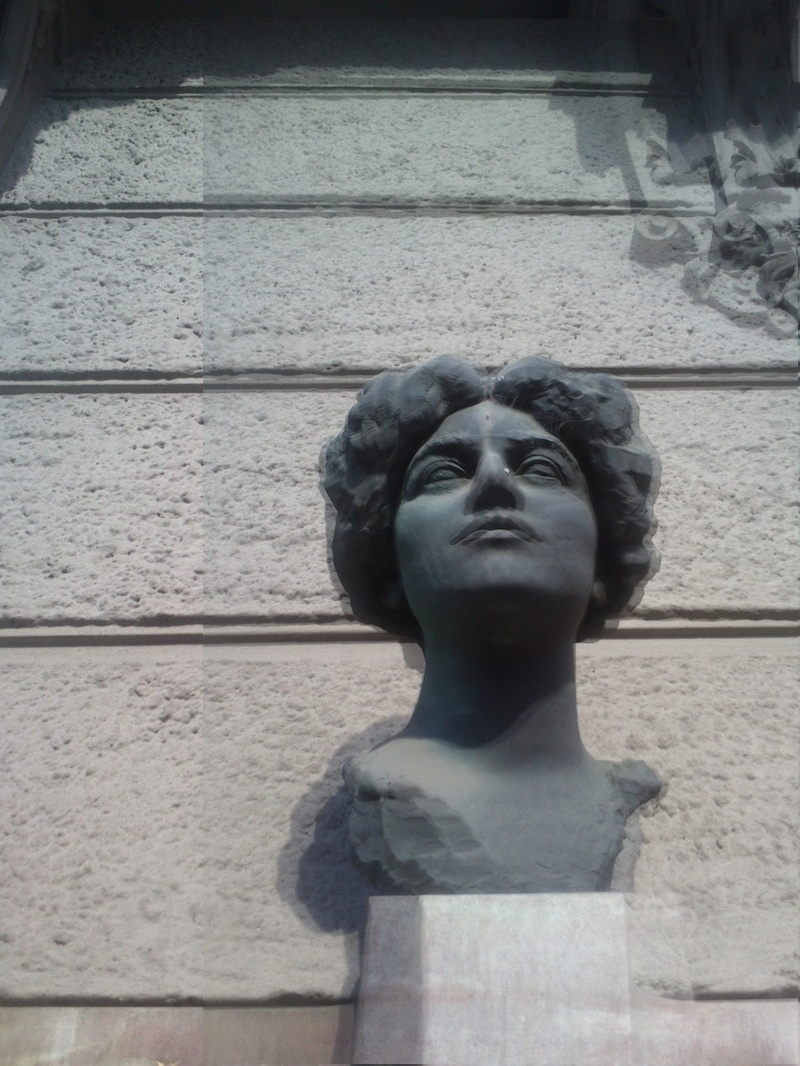
\includegraphics[width=4.5cm]{img/ema_overlap.png}
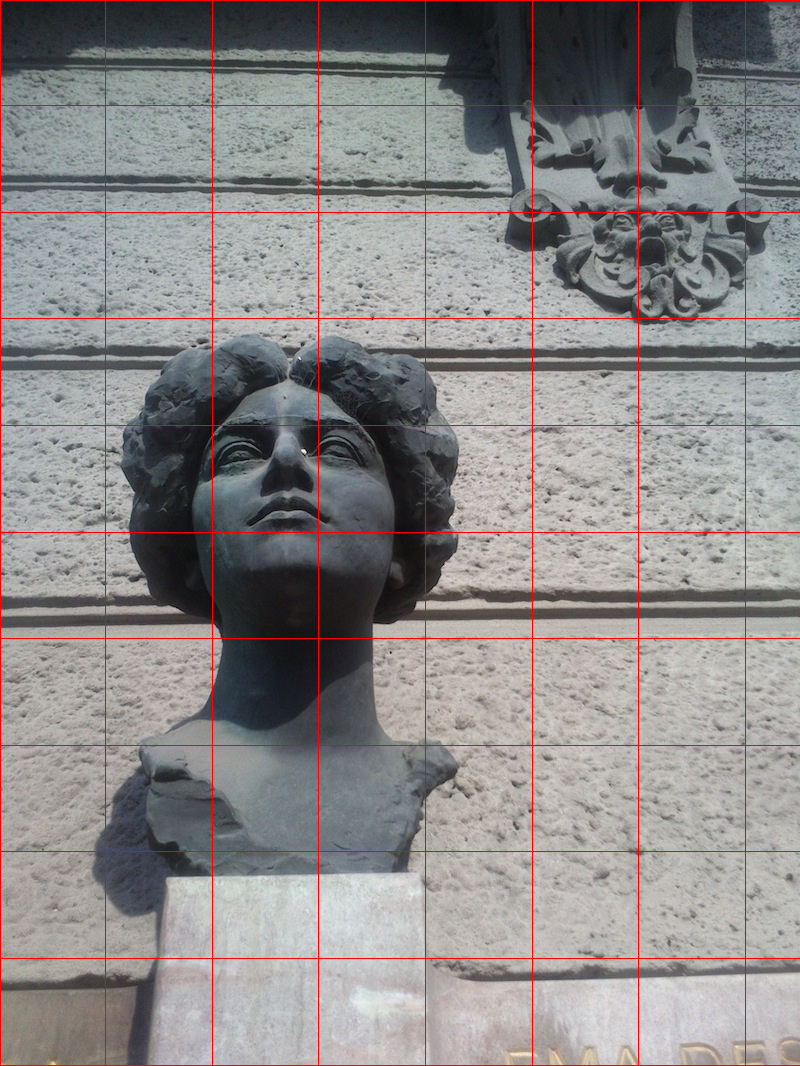
\includegraphics[width=4.5cm]{img/ema_buckets.png}}
\caption{Left: The result of the registration where the process of upscaling was stopped when the height of the image was over 200px. Right: The division of an image into square-boxes.}
\label{fig:overlap}
\end{figure}

The next step of the process is detection of keypoints which are detected with the SURF detector.
We divide the images into square-boxes of the same size and to each square-box we assign an array of keypoints situated in it.
Because of the previous calculation of approximate overlap we do not have to match all keypoints in the image, but we choose only the keypoints lying in the overlap.
To identify the relative position of the image pair better we detect the most robust keypoint match from our SURF keypoint set and calculate the vector defining the direction of the shift of the keypoint.
To find this robust match we choose only the keypoints with response higher than 4000 and %match them with the SURF keypoints detected in the second image.
%Each corresponding point we search only in the 30 $\times$ 30 pixels area around the estimated presence of the match calculated from the relative position.
each of them we try to match with one keypoint extracted in the second image but only in the corresponding 30 $\times$ 30 pixels area determined due the previous image registration.
To decrease the computational time we use the pre-calculated square-boxes to find the keypoints of the second image lying in this area.
To avoid mismatches we reject the matches where the matched keypoints differs too much in the orientation or if there are more than one obvious potential points for the match.

\begin{figure}[h]
\centerline{
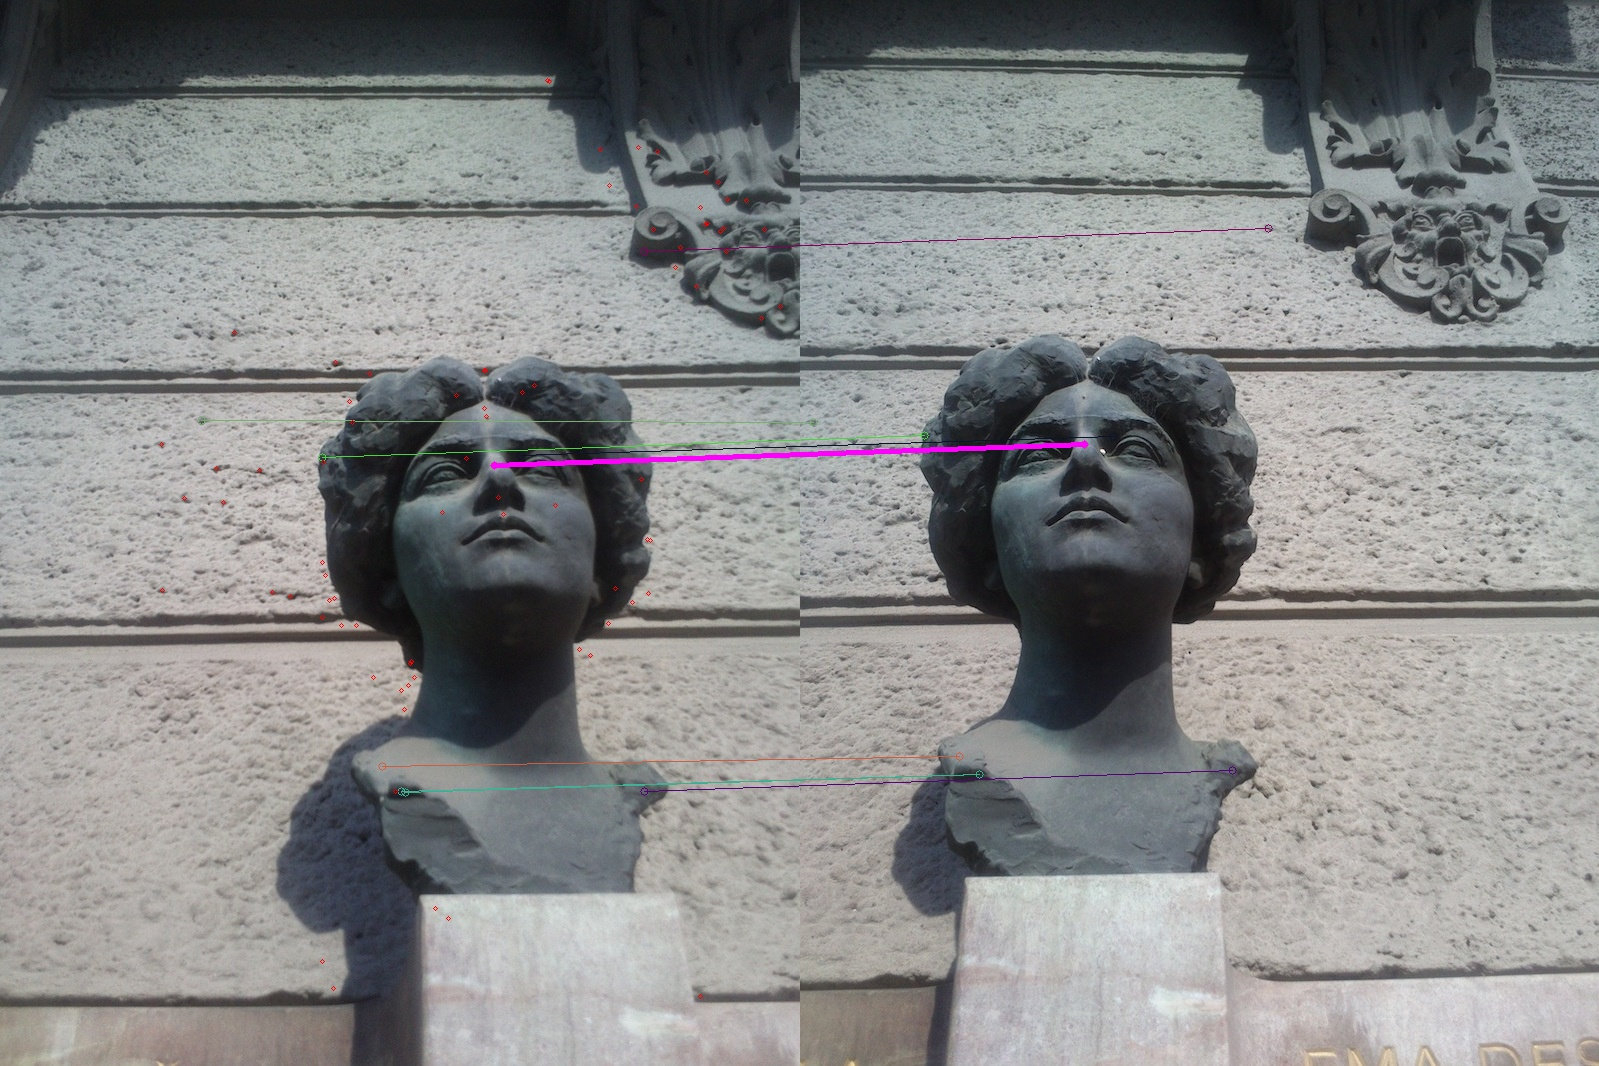
\includegraphics[width=9cm]{img/ema_direction.png}}
\caption{The most robust match chosen from the keypoints with response higher than 4000. According to this match the more accurate relative position of images is estimated.}
\label{fig:overlap}
\end{figure}

When we know the more accurate relative position of the images, we investigate the keypoints one more time.
Now we iterate all of them. 
Each keypoint in the first image we try to match with a keypoint in the estimated corresponding surrounding area in the second image in the shape of oriented rectangle computed based on the more accurate relative image position.
% and try to match them in the corresponding area in the shape of oriented rectangle.
Matched keypoints which differs too much in the orientation or are not obviously the best match we reject again.

%Dense correspondence: optical flow::
At this point we have relatively robust matches for sparse correspondence. 
For the calculation of the depth information we need to extract more corresponding points.
For this purpose we use optical flow algorithm. 
For each SURF keypoint in the first image we detect corners or other features acceptable for the tracking algorithm in its 70 $\times$ 70 pixels area.

\begin{figure}[h]
\centerline{
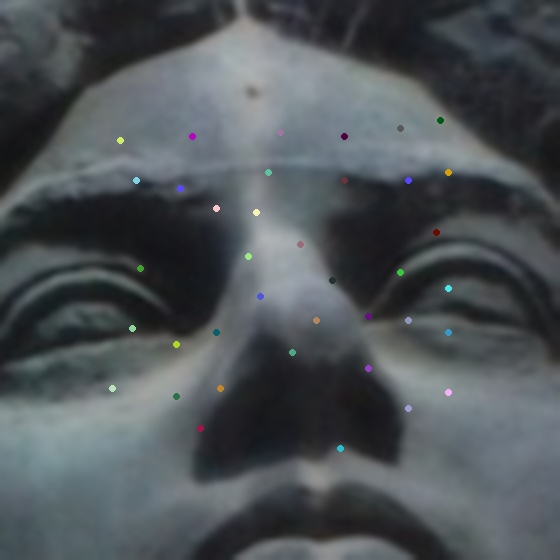
\includegraphics[width=6.0cm]{img/trackingpoints1a.png}
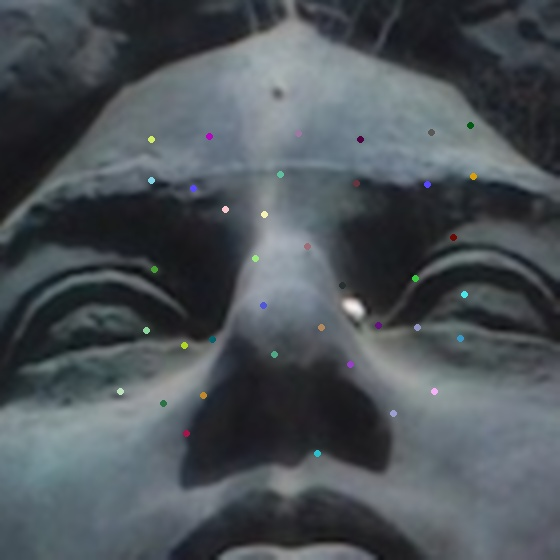
\includegraphics[width=6.0cm]{img/trackingpoints2a.png}}
\caption{70 $\times$ 70 windows of the pair of the input images with optical flow matches.}
\label{fig:trackingpoints}
\end{figure}

Calculating the optical flow we get the corresponding points in the second image.
With high probability some of the results will be influenced by noise.
To avoid these mismatches we calculate the variation of the distances between each match.
If the variation is higher than 300 we discard all of the detected optical flow matches.

The result is visualized in OpenGL ES.
Every keypoint is represented as a triangle in a space with the depth calculated from the correspondence.
At first, the user can view the rough model created from the results of SURF matching.
Each time some of the dense corresponding points are calculated with optical flow algorithm, the model is updated.

\section{Project structure}
The project resources can be divided into four parts:
\begin{itemize}
\item{Activities, }
\item{Classes, }
\item{Structures, }
\item{xml files defining layout and other files in the /res folder.}
\end{itemize}


